{\tmstrong{Objective: Solve systems of equations by graphing and identifying
the point of intersection. }}\pp

We have solved problems like $3 x - 4 = 11$ by adding 4 to both sides and then
dividing by 3 (solution is $x = 5$). We also have methods to solve equations
with more than one variable in them. It turns out that to solve for more than
one variable we will need the same number of equations as variables. For
example, to solve for two variables such as $x \tmop{and} y$ we will need two
equations. When we have several equations we are using to solve, we call the
equations a {\tmstrong{system of equations}}. When solving a system of
equations we are looking for a solution that works in each equation simultaneously. This
solution is usually given as an ordered pair $(x, y)$. The following example
illustrates a solution working in two equations.\pp

%\vspace{1.5in}
%~\\

\begin{example}~~~
  Show ($x,y$)=(2,1) is the solution to the system
\begin{center}
	%$\begin{array}{l}
   $ 3 x - y = 5$~~~~~~~$x + y = 3$
  %\end{array}$
\end{center}
	\begin{eqnarray*}
    (x,y)=(2, 1) &  & \tmop{Identify} x \tmop{and} y \tmop{from} \tmop{the}
    \tmop{ordered} \tmop{pair}\\
    x = 2,~y = 1 &  & \tmop{Plug} \tmop{these} \tmop{values} \tmop{into}
    \tmop{each} \tmop{equation}%\\
	\end{eqnarray*}
	\begin{eqnarray*}
%    &  & \\
    3 (2) - (1) = 5 &  & \tmop{First} \tmop{equation}\\
    6 - 1 = 5 &  & \tmop{Evaluate}\\
    5 = 5 &  & \tmop{True}\\
    &  & \\
    (2) + (1) = 3 &  & \tmop{Second} \tmop{equation}, \tmop{evaluate}\\
    3 = 3 &  & \tmop{True}
  \end{eqnarray*}
\end{example}

As we found a true statement for both equations we know (2,1) is the solution
to the system. It is in fact the only combination of numbers that works in
both equations.  In this section, we will attempt to identify a (simultaneous) solution to two equations, if such a solution exists.  It stands to reason that if we use points to describe the solution, we can use graphs to find the solution.\pp
If the graph of a line is a picture of all the solutions to its equation, we can graph two
lines on the same coordinate plane to see the solutions of both equations. In particular, we
are interested in finding all points that are a solution for both equations.  This will be
the point(s) where the two lines intersect! If we can find the intersection of the lines we
have found the solution that works in both equations.%\pp

%\vspace{1in}
%~\\

\begin{example}~~~Solve the following system of equations.
  
  \begin{eqnarray*}
    \begin{array}{l}
      y = - \frac{1}{2} x + 3\\
    	y = \frac{3}{4} x - 2
   \end{array} &  & \tmop{First} \tmop{identify}
    \tmop{slopes} \tmop{and} y - \tmop{intercepts}\\
  & & \\ 
	\begin{array}{l}
      \tmop{First~Line} : ~~~m = - \frac{1}{2}, ~~b = 3\\
      \tmop{Second~Line} : ~m = \frac{3}{4}, ~~~b = - 2
    \end{array} &  & \tmop{Next} \tmop{graph} \tmop{both}
    \tmop{lines} \tmop{on} \tmop{the} \tmop{same} \tmop{plane}\\
  \end{eqnarray*}
  
%	\vspace{1in}
%	~\\
	
	\begin{multicols}{2}
    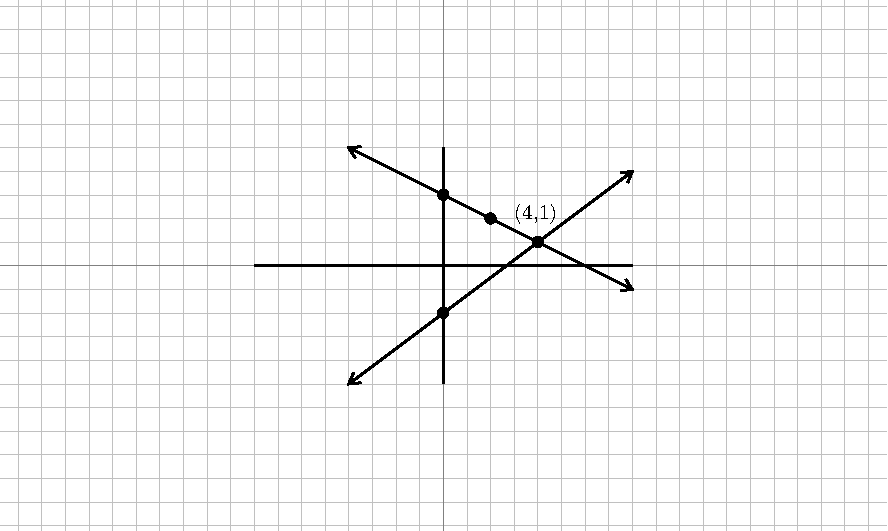
\includegraphics[scale=.85,bb = 115 65 310 190, clip=true]{II_2_1-1.eps}
    
    To graph each equation, we start at the $y$-intercept and use the slope
    ($\frac{\tmop{rise}}{\tmop{run}}$) to get the next point, then connect the
    dots.\pp
		Remember a line with a negative slope points downhill from left to right!
  \end{multicols}
    \begin{center}
    Find the intersection point, (4,1).  This is our solution.
		\end{center}
\end{example}


Often our equations won't be in slope-intercept form and we will have to solve
both equations for $y$ first so we can identify the slope and $y$-intercept.

\begin{example}~~~Solve the following system of equations.
  \begin{eqnarray*}
    \begin{array}{l}
      6 x - 3 y = - 9\\
      2 x + 2 y = - 6
    \end{array} &  & \tmop{Solve} \tmop{each} \tmop{equation} \tmop{for~} y\\
    %&  & \\
	\end{eqnarray*}
	\begin{eqnarray*}
	6 x - 3 y = - 9~~ & ~~~~~~2 x + 2 y = - 6~~~ &\\
    \tmmathbf{\underline{- 6 x ~~~~~~~- 6 x}} & ~~~\tmmathbf{\underline{- 2 x ~~~~~~~~- 2 x}} &  \tmop{Subtract~} x
    \tmop{~terms}\\
    &  & \\
		- 3 y = - 6 x ~- 9 & ~~~2 y = - 2 x - 6 & \tmop{Rearrange} \tmop{equations}\\
    \tmmathbf{\overline{- 3} ~~~~~ \overline{- 3} ~~ \overline{- 3}} & ~~~\tmmathbf{\overline{2} ~~~~~~~ \overline{2} ~~~~~ \overline{2}} & \tmop{Divide} \tmop{by} \tmop{coefficient} \tmop{of~}
    y\\
		&  & \\
    y = 2 x + 3~~~ & ~~~y = - x - 3 &\tmop{Identify} \tmop{slope} \tmop{and~} y -
    \tmop{intercepts}%\\
		%& & \\
	\end{eqnarray*}
	\begin{eqnarray*}
    \begin{array}{l}
			\tmop{First~Line} : ~~~~m = \frac{2}{1}, ~~~~b = 3\\
      \tmop{Second~Line} : ~m = - \frac{1}{1}, ~~b = - 3
    \end{array} &  & \tmop{Next} \tmop{graph} \tmop{both}
    \tmop{lines} \tmop{on} \tmop{the} \tmop{same} \tmop{plane}\\
		%& & \\
  \end{eqnarray*}
  \begin{multicols}{2}
    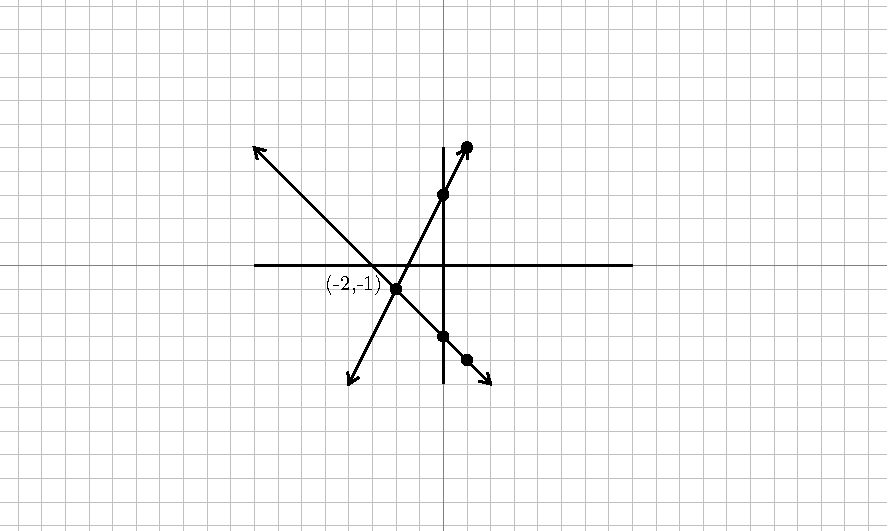
\includegraphics[scale=.85,bb = 115 65 310 190, clip=true]{II_2_1-2.eps}
    
    To graph each equation, we start at the $y$-intercept and use the slope
    ($\frac{\tmop{rise}}{\tmop{run}}$) to get the next point, then connect the
    dots.\pp
    
    Remember a line with a negative slope points downhill from left to right!
  \end{multicols}
    \begin{center}
    Find the intersection point, (-2,11).  This is our solution.
		\end{center}
\end{example}


As we are graphing our lines, it is possible to have one of two unexpected
results. These are shown and discussed in the next two examples.\pp

\vspace{1in}
~\\

\begin{example}~~~Solve the following system of equations.
    \begin{center}
			%\begin{array}{l}
      $y = \frac{3}{2} x - 4$ ~~~~~~~~~~~~~~ $y = \frac{3}{2} x + 1$\pp
%			\end{array} 
		%&  & \tmop{Identify} \tmop{slope} \tmop{and} y -
    %\tmop{intercept} \tmop{of} \tmop{each} \tmop{equation}\\
    %& & \\
		Identify the slope and $y-$intercept of each equation.
		\end{center}
  \begin{eqnarray*}
		\begin{array}{l}
			\tmop{First~Line} : ~~~~m = \frac{3}{2}, ~~b = -4\\
      \tmop{Second~Line} : ~m = \frac{3}{2}, ~~b = 1
    \end{array} &  & \tmop{Next} \tmop{graph} \tmop{both}
    \tmop{lines} \tmop{on} \tmop{the} \tmop{same} \tmop{plane}\\
		%& & \\
	\end{eqnarray*}
  \begin{multicols}{2}
    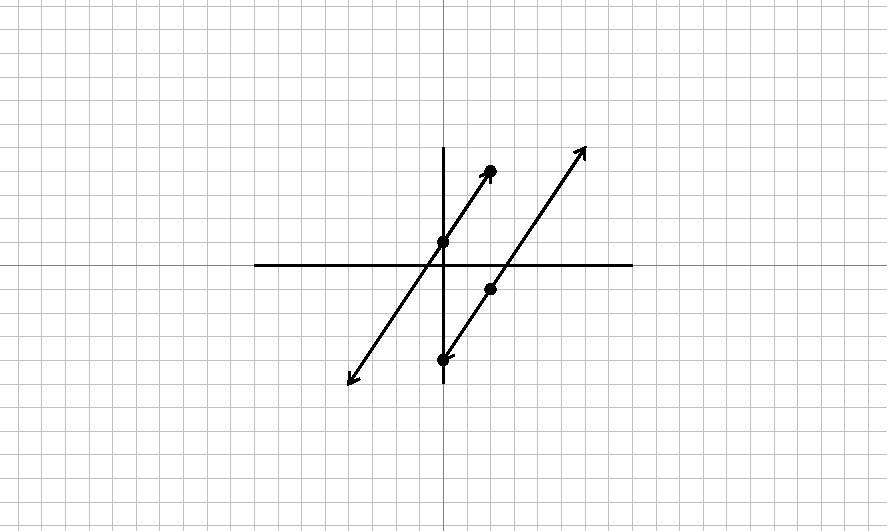
\includegraphics[scale=.85,bb = 115 65 310 190, clip=true]{II_2_1-3.eps}

%~\pp
%~\par

    To graph each equation, we start at the $y$-intercept and use the slope
    ($\frac{\tmop{rise}}{\tmop{run}}$) to get the next point, then connect the
    dots.\pp
    
    The two lines do not intersect; they are parallel!
	\end{multicols}
	 Since the lines do not intersect, we know that there is no point that will satisfy both equations.  
		\begin{center}    
    There is no solution, or $\varnothing$.
		\end{center}
\end{example}
~\par  
Notice that we could also have recognized that both lines had the same slope. Remembering
that parallel lines have the same slope one could conclude that there is no
solution without having to graph the lines.\pp

\vspace{1in}
~\\

\begin{example}~~~Solve the following system of equations.
  \begin{eqnarray*}
    \begin{array}{l}
      2 x - 6 y = 12\\
      3 x - 9 y = 18
    \end{array} &  & \tmop{Solve} \tmop{each} \tmop{equation} \tmop{for~} y
    %&  & \\
	\end{eqnarray*}
	\begin{eqnarray*}
    2 x - 6 y = 12~~~ &~~~3 x - 9 y = 18~~ &\\
    \tmmathbf{\underline{- 2 x ~~~~~~~- 2 x}} &~~~ \tmmathbf{\underline{- 3 x ~~~~~~~- 3 x}} &\tmop{Subtract} x
    \tmop{terms}\\
		& & \\
    - 6 y = - 2 x + 12 &~~~ - 9 y = - 3 x + 18~ & \tmop{Put} x \tmop{terms}
    \tmop{first}\\
    \tmmathbf{\overline{- 6} ~~~~~ \overline{- 6} ~~~ \overline{- 6}} &~~~ \tmmathbf{\overline{- 9}~~~~~ 
    \overline{- 9} ~~~ \overline{- 9}} & \tmop{Divide} \tmop{by}
    \tmop{coefficient} \tmop{of} y\\
    y = \frac{1}{3} x - 2~~~ &~~~ y = \displaystyle\frac{1}{3} x - 2 & \tmop{Identify}
    \tmop{the} \tmop{slopes} \tmop{and} y - \tmop{intercepts}\\
	\end{eqnarray*}
	\begin{eqnarray*}
    \begin{array}{l}
			\tmop{First~Line} : ~~~~m = \frac{1}{3}, ~~b = -2\\
      \tmop{Second~Line} : ~m = \frac{1}{3}, ~~b = - 2
    \end{array} &  & \tmop{Next} \tmop{graph} \tmop{both}
    \tmop{lines} \tmop{on} \tmop{the} \tmop{same} \tmop{plane}\\
		%& & \\
  \end{eqnarray*}
  \begin{multicols}{2}
    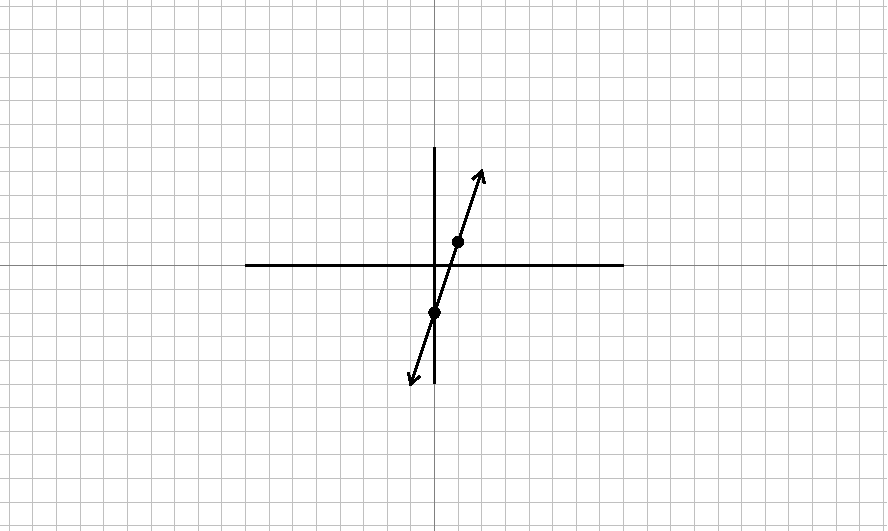
\includegraphics[scale=.85,bb = 115 65 310 190, clip=true]{II_2_1-4.eps}
    
    To graph each equation, we start at the $y$-intercept and use the slope
    ($\frac{\tmop{rise}}{\tmop{run}}$) to get the next point, then connect the
    dots.\pp
    
    Both equations are the same line! 
 	\end{multicols}
As one line is directly on top of the other line, we can say that the lines ``intersect'' everywhere!
		\begin{center}    
    Here we say there are infinitely many solutions.\\
		\end{center}
\end{example}
  
Notice that once we had both equations in slope-intercept form we could have recognized that
the equations were the same. At this point one could state that there are
infinitely many solutions without having to go through the work of graphing the
equations.\pp

{\tmstrong{World View Note: }}The Babylonians were the first to work with
systems of equations with two variables. However, their work with systems was
quickly passed by the Greeks who would solve systems of equations with three
or four variables and around 300 A.D., developed methods for solving systems
with any number of unknowns!

%\end{document}
